\documentclass[a4paper,12pt]{article}

\usepackage[utf8]{inputenc}
\usepackage{geometry}
\usepackage{graphicx}
\usepackage{amsmath}
\usepackage{hyperref}

\geometry{margin=1in}

\title{Electronics Experiment Report: Diode Characteristics}
\author{B13901165張勝勛, B13901087洪秉軒}
\date{\today}

% Language and font packages
\usepackage{ctex} % Chinese support

% Pseudocode and algorithm packages
% \usepackage{algorithm2e} % Advanced algorithm writing
% \usepackage{algpseudocode} % Pseudocode environment for algorithms

% Fancy style packages
\usepackage{fancyhdr} % Custom headers/footers
\usepackage{color} % Color support
\usepackage{xcolor} % Extended color support
\usepackage{tcolorbox} % Colored boxes
\usepackage{framed} % Framed environments

% Math and symbol packages
\usepackage{amsfonts}
\usepackage{amssymb}
\usepackage{mathtools}

% Table and figure packages
% \usepackage{booktabs} % Professional tables
% \usepackage{multirow} % Multi-row tables
% \usepackage{caption} % Custom captions
\usepackage{subcaption} % Subfigures

% Miscellaneous
\usepackage{enumitem} % Custom lists
\usepackage{listings} % Code listings
\usepackage{tikz} % Drawing diagrams
\usepackage{pgfplots} % For plotting graphs
\usepackage{float}

\begin{document}

\maketitle

\section{Electrical Properties of Diodes}
in this section, we  connect a diode(Si or zener) and a resistance in series and observe the output waveform and estimate the cut-in voltage
of the diode
\subsection{setup}
\begin{itemize}
    \item $V_s$ = 6sin(2$\pi$ft)V for Si diode
    \item $V_s$ = 10sin(2$\pi$ft)V for zener diode
    \item $R_L$ = 10k$\Omega$
\end{itemize}
\begin{figure}[H]
    \centering
    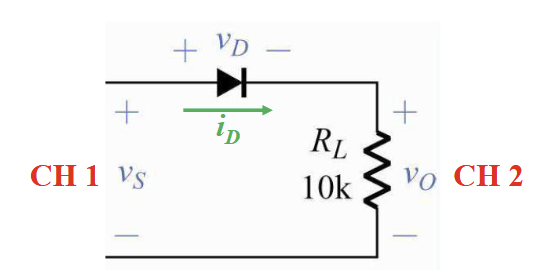
\includegraphics[width=0.5\textwidth]{exp1.png}
    \caption{the circuit diagram for the first experiment}
\end{figure}
\subsection{graph}
\begin{figure}[H]
    \centering
    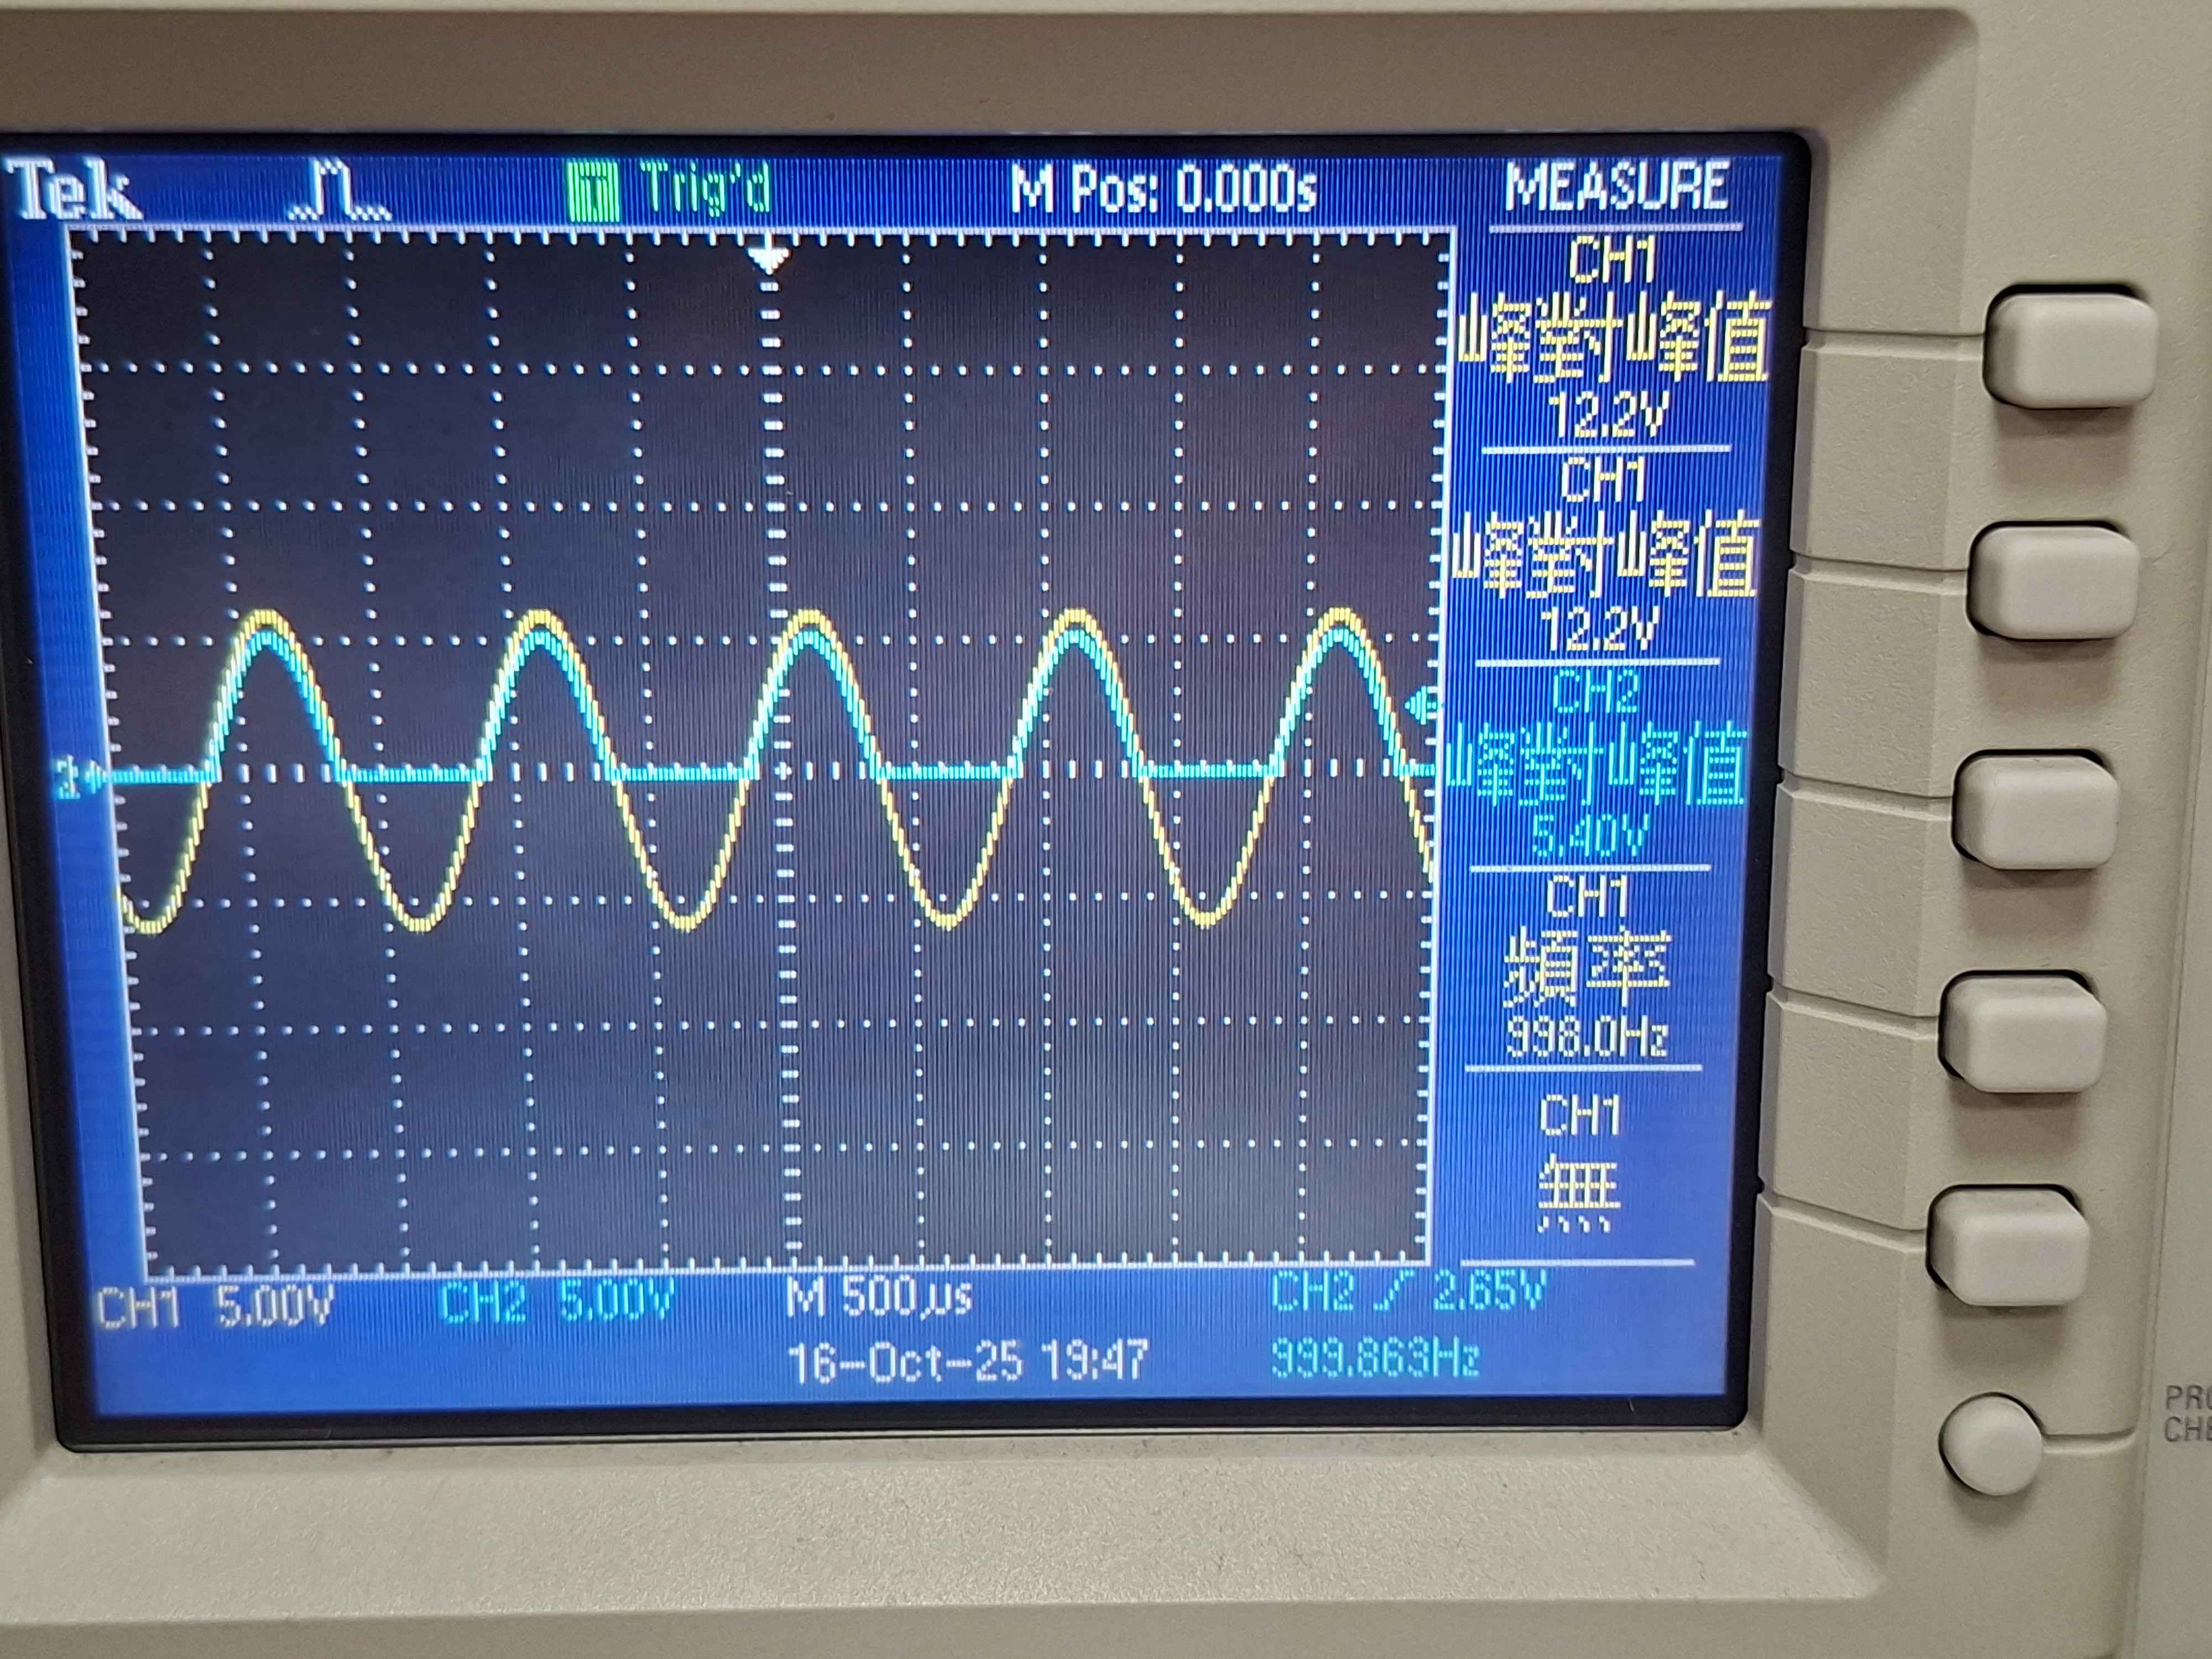
\includegraphics[width=0.8\textwidth]{Si_1k.jpg}
    \caption{the output waveform of Si diode with 1k resistance}
\end{figure}
\begin{figure}[H]
    \centering
    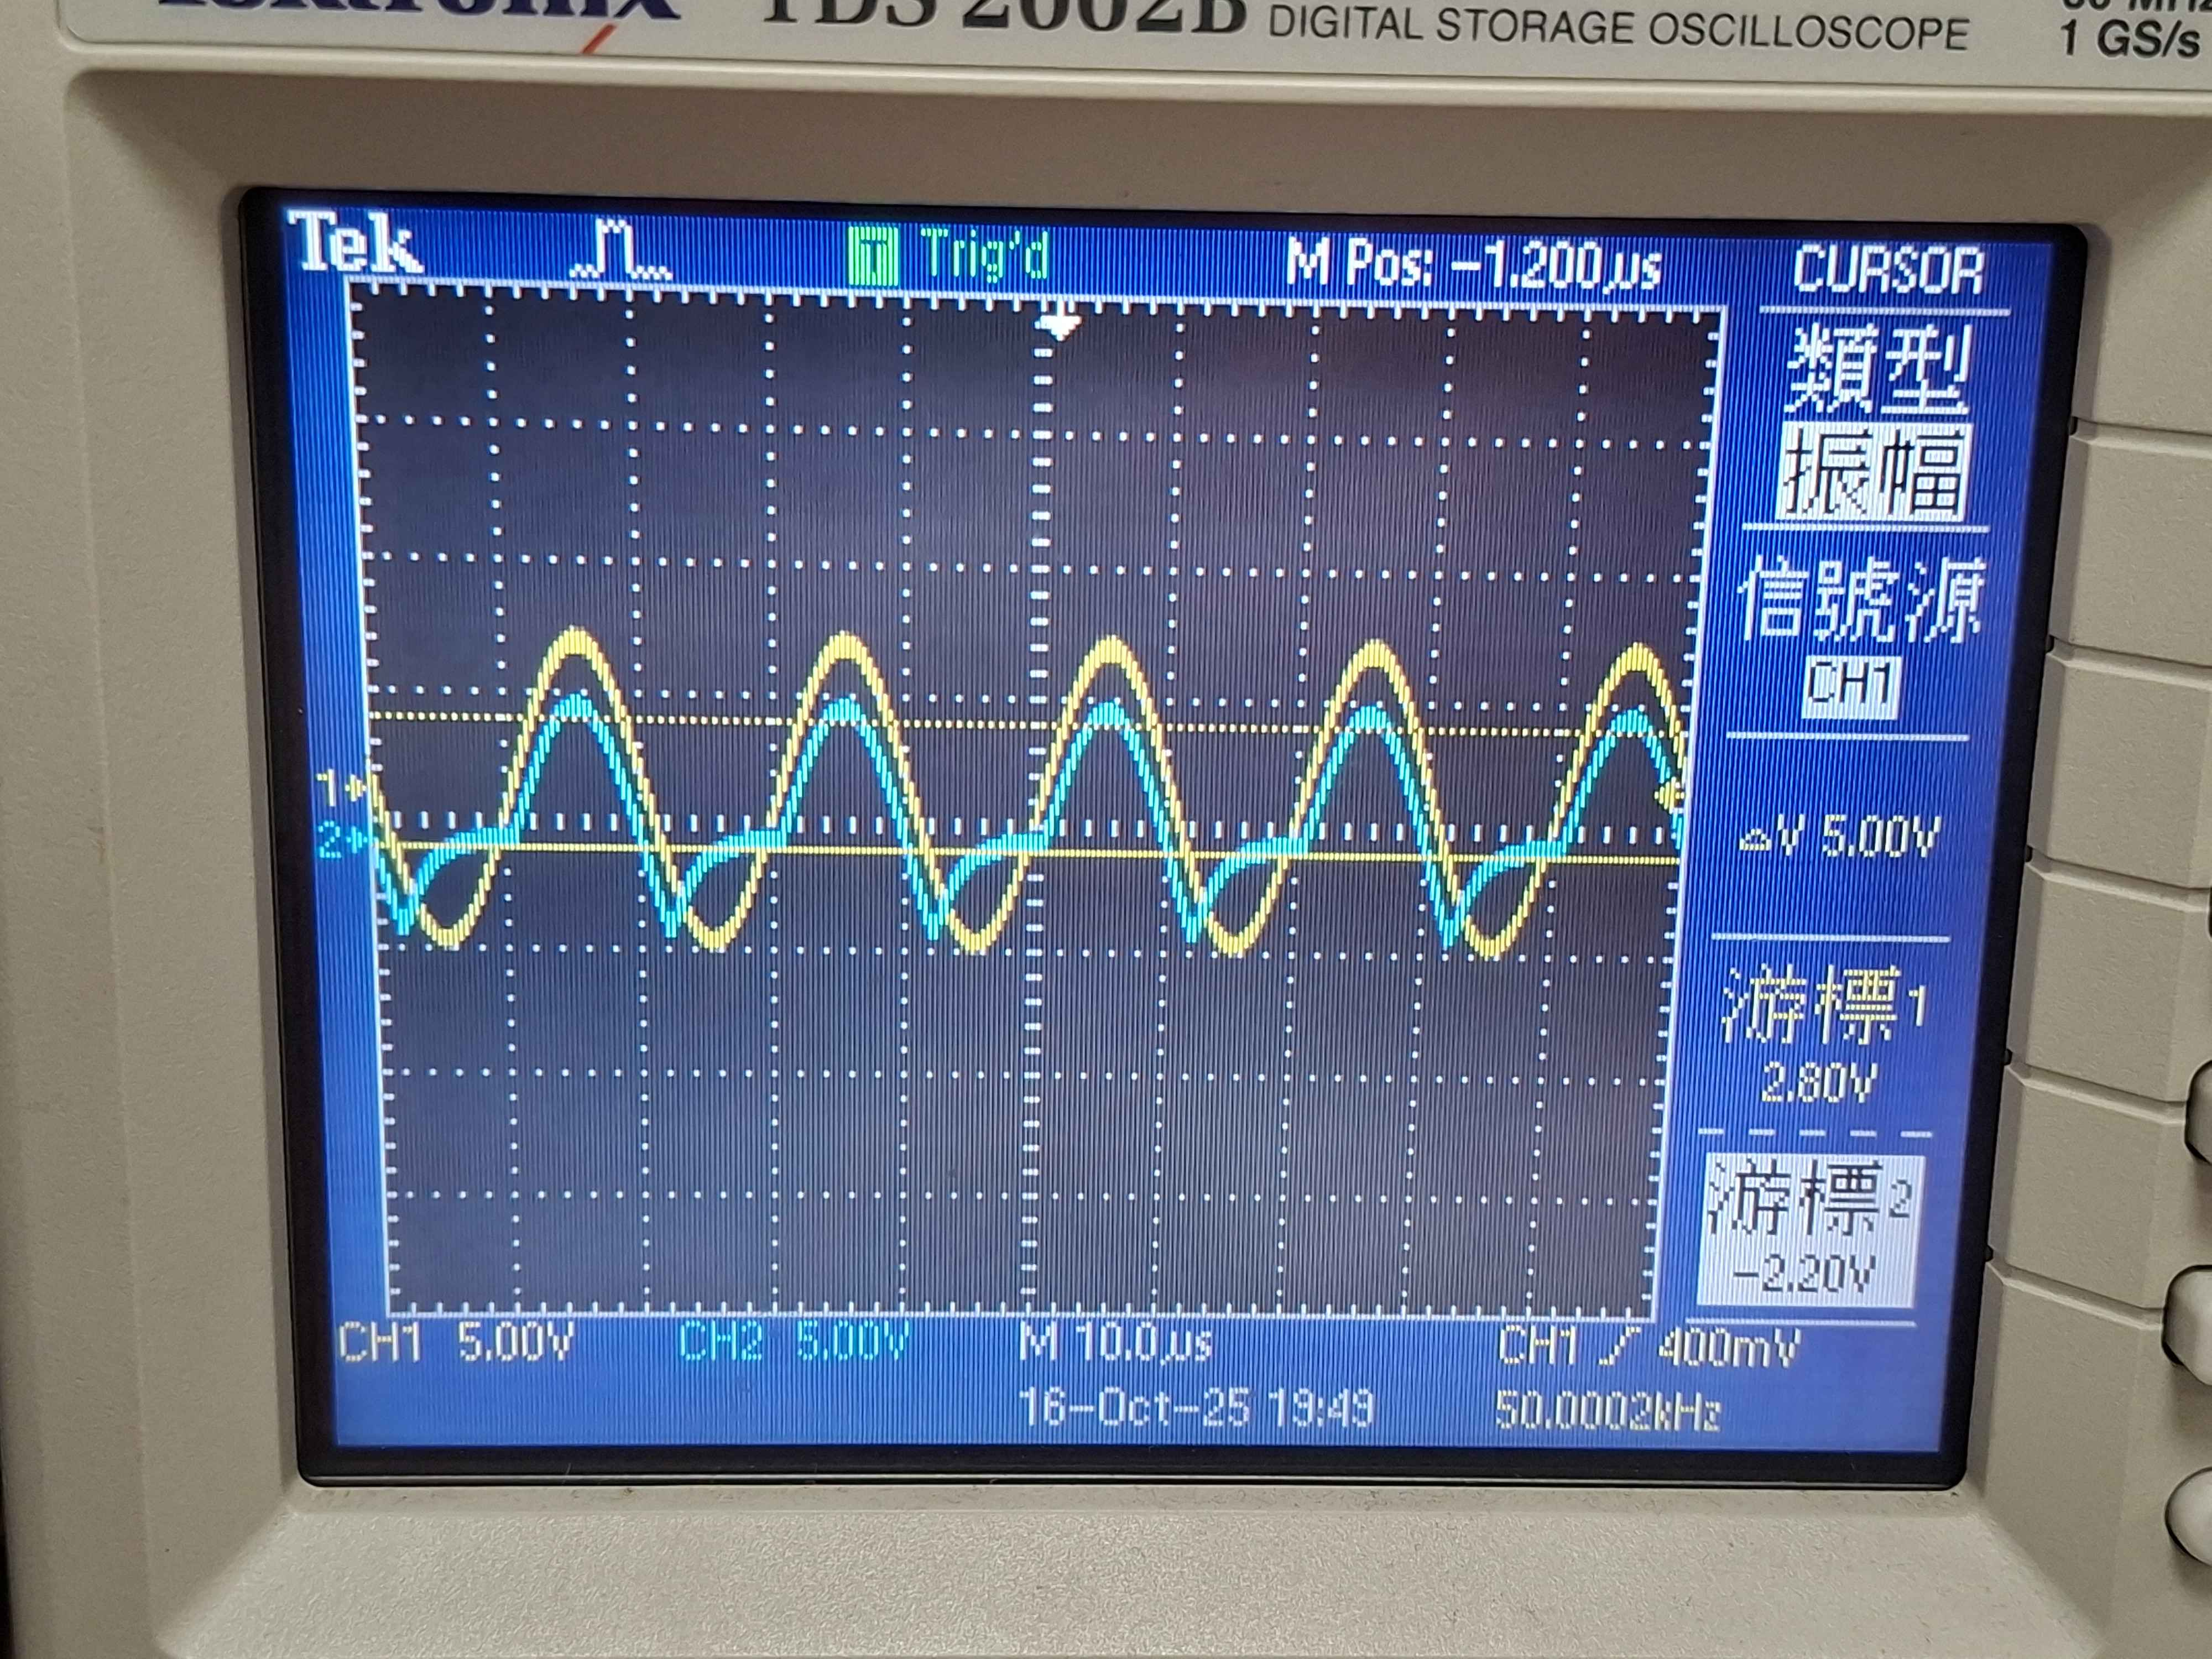
\includegraphics[width=0.8\textwidth]{Si_50k.jpg}
    \caption{the output waveform of Si diode with 50k resistance}
\end{figure}
\begin{figure}[H]
    \centering
    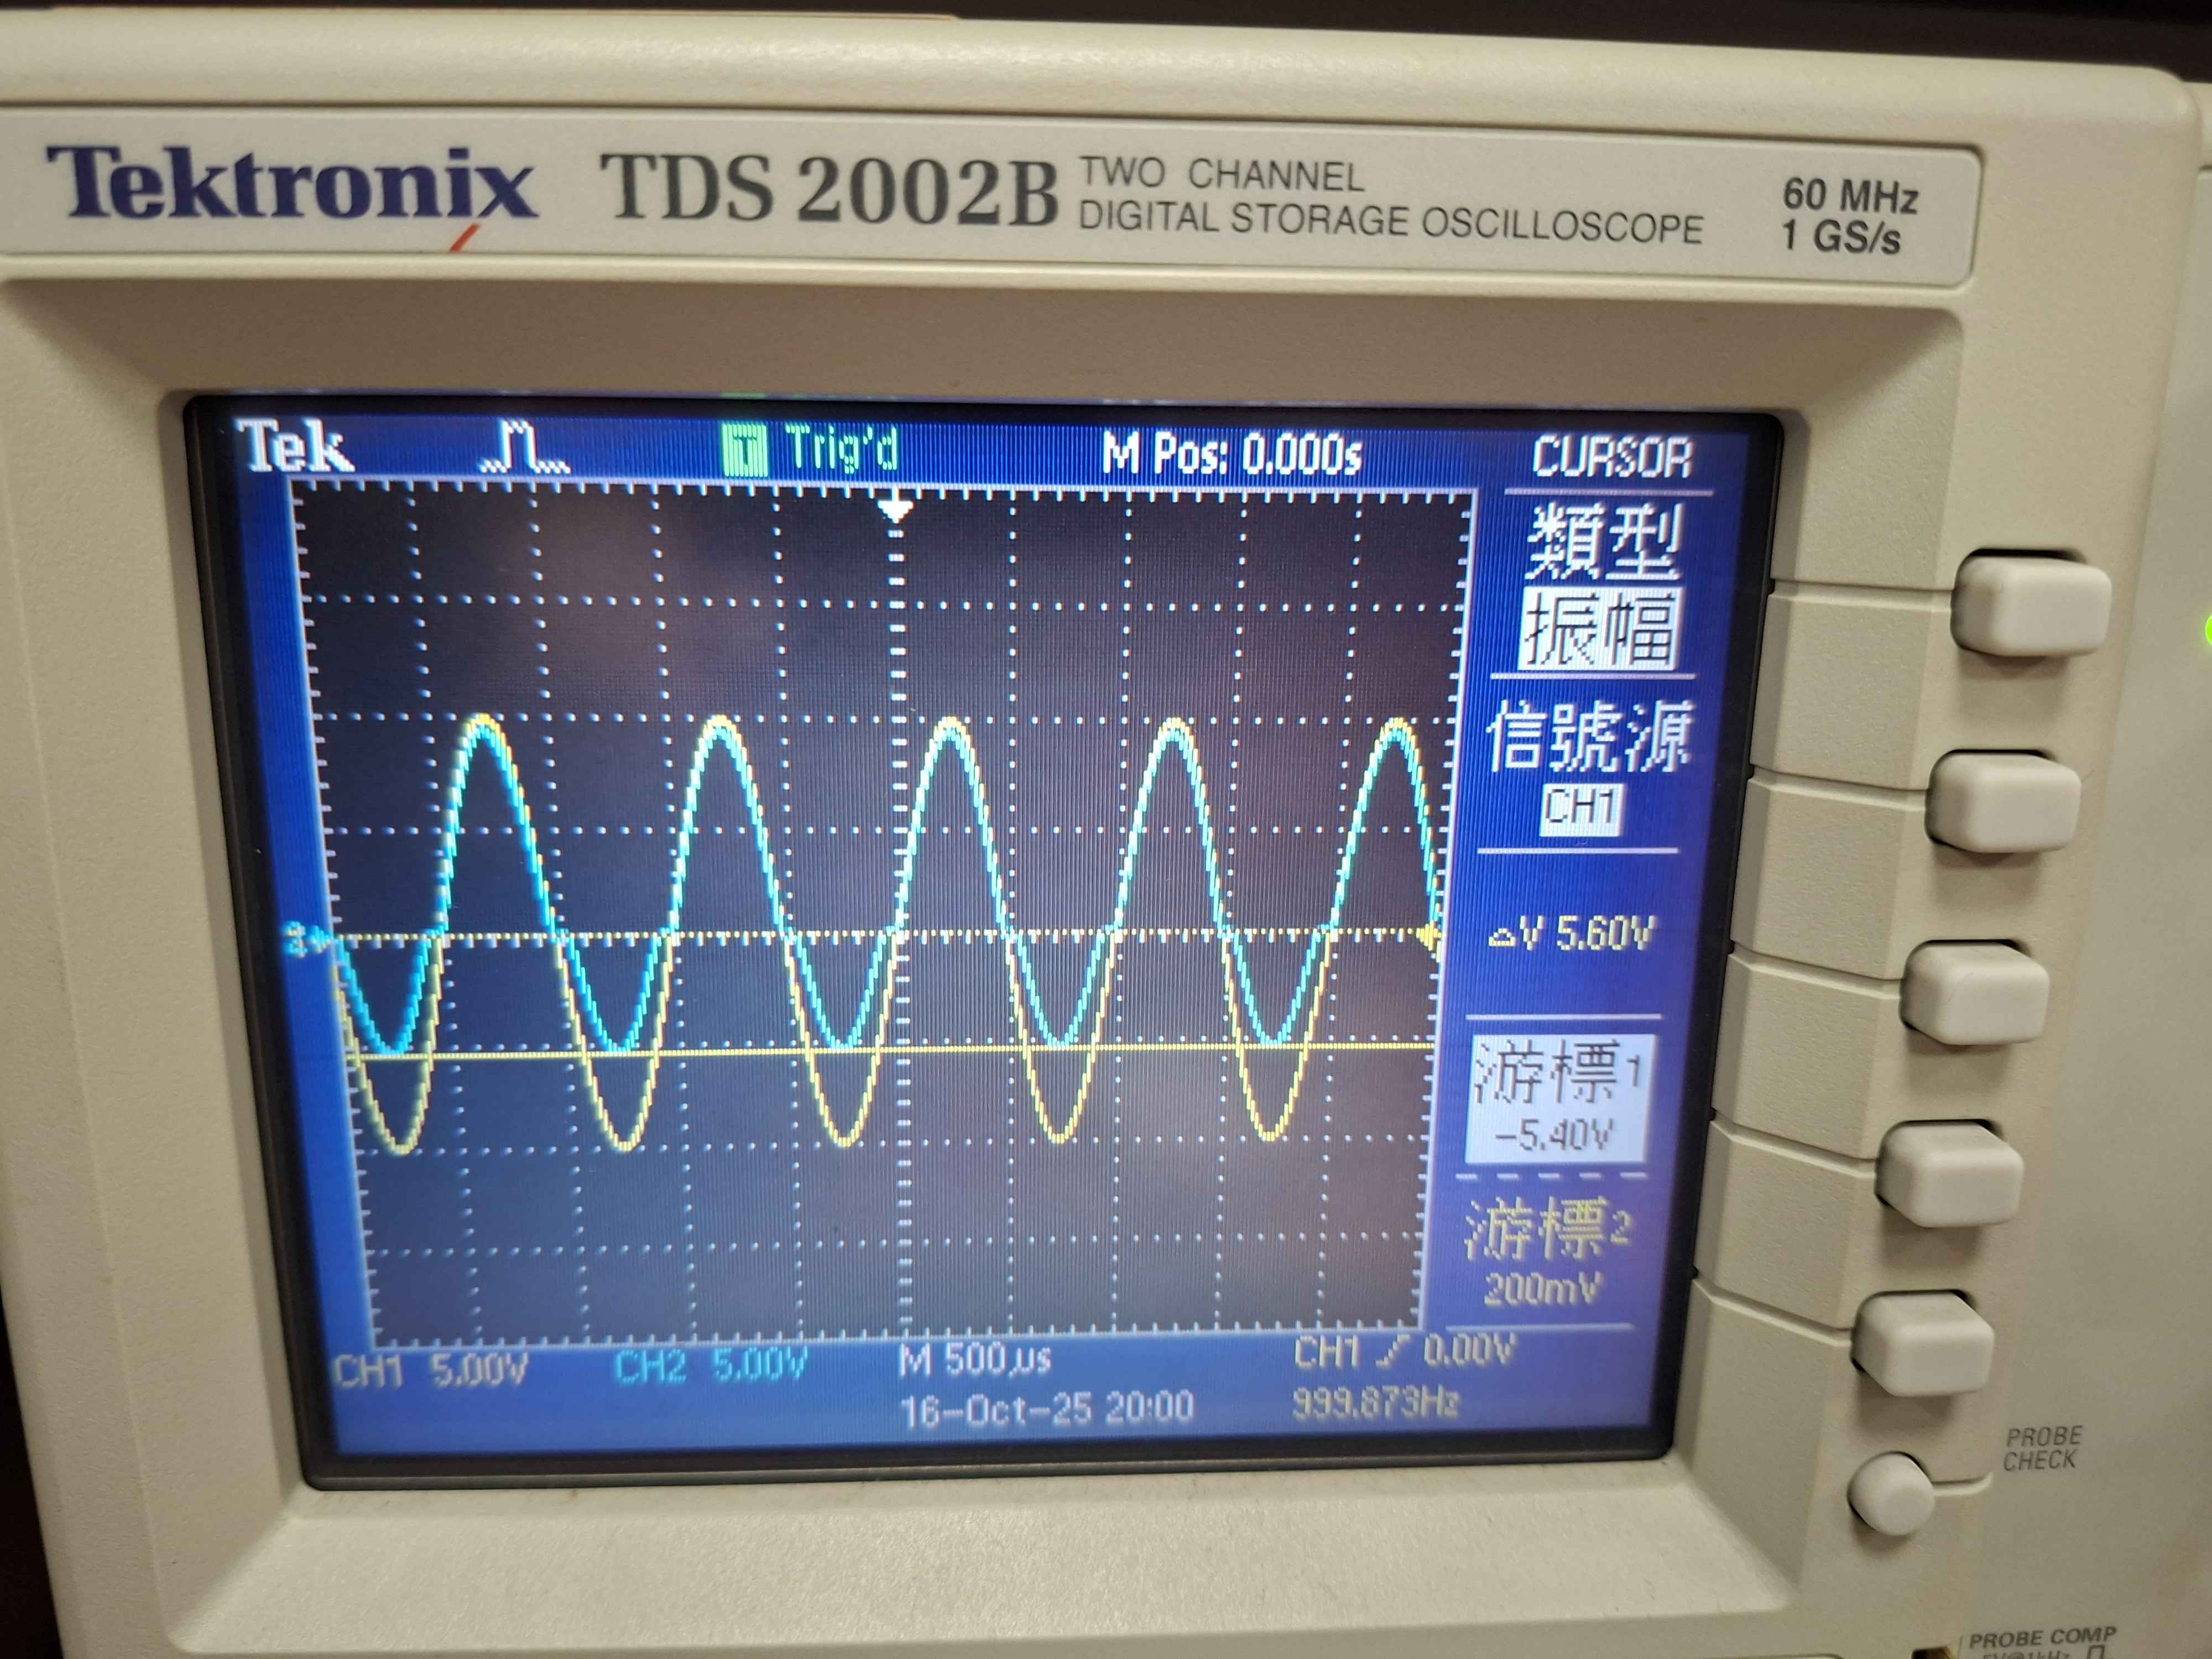
\includegraphics[width=0.8\textwidth]{zener_1k.jpg}
    \caption{the output waveform of zener diode with 1k resistance}
\end{figure}
\subsection{$V_D$and $V_Z$}
\begin{enumerate}
    \item For Si diode, since CH1's peak voltage is 6.1V and CH2's peak voltage is 5.4V, 
    we can estimate the cut-in voltage $V_D$ as: 6.1V - 5.4V = 0.7V
    \item For zener diode, since in the negative half cycle, the peak voltage difference is about 5.6V, 
    we can estimate the zener voltage $V_Z$ as: 5.6V
\end{enumerate}

\section{Voltage Regulator}
\subsection{setup}
\begin{itemize}
    \item $R_1$ = 10k$\Omega$
    \item $V_i$ = 9V DC
\end{itemize}
\begin{figure}[H]
    \centering
    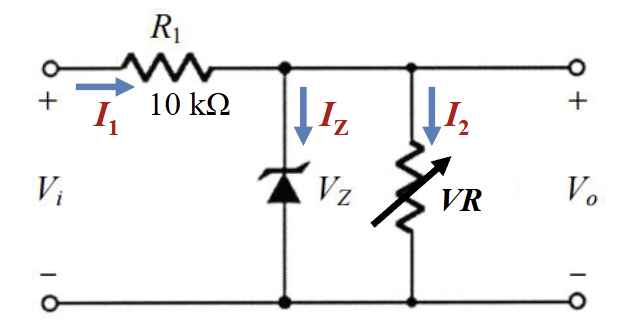
\includegraphics[width=0.5\textwidth]{exp2.png}
    \caption{the circuit diagram for the second experiment}
\end{figure}
\subsection{Experiment result}
\begin{table}[H]
    \centering
    \begin{tabular}{|c|c|c|c|c|}
        \hline
        $R_L$ & $I_1$  & $I_Z$ & $I_2$ & $V_o$  \\
        \hline
        2k$\Omega$ & 0.758mA & 0mA & 0.758mA & 1.5V \\
        50k$\Omega$ & 0.477mA & 0.391mA & 0.085mA & 4.27V \\
        400k$\Omega$ & 0.472mA & 0.462mA & 0.011mA & 4.32V \\
        800k$\Omega$ & 0.472mA & 0.467mA & 0.004mA & 4.32V \\

        \hline
    \end{tabular}
    \caption{Output voltage and zener current for different load resistances}
\end{table}
\subsection{conclusion}
\begin{itemize}
    \item When $R_L$ is small (about 2k$\Omega$), $I_Z$ is 0, indicating that the zener diode is not regulating the voltage. so the output
    voltage is about $\frac{2k}{10k+2k}$ $\cdot$ $9V = 1.5V$
    \item As $R_L$ increases, the output voltage approaches the zener voltage, the output voltage is about 4.3V
\end{itemize}

\end{document}